\subsection{Segregation system}

\subsubsection{Check data balancing}

\begin{figure}[H]
\centering
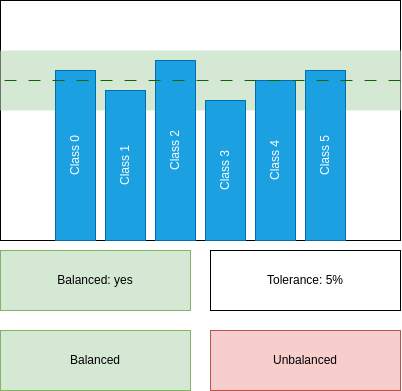
\includegraphics[width=0.8\textwidth]{figures/check_data_balancing.png}
\caption{"Check data balancing" mock-up form}
\end{figure}

\begin{table}[H]
\centering
\begin{tabularx}{\textwidth}{|X|c|c|c|c|}
\hline
\textbf{Step} & \textbf{O} & \textbf{CL} & \textbf{S} & \textbf{SC} \\
\hline
\textbf{1} \textbf{ACTOR} opens "Check data balancing" form. & & & & \\
\hline
\textbf{2} \textbf{SYSTEM} shows the report. & & & & \\
\hline
\textbf{3} \textbf{SYSTEM} shows a hint whether the data is balanced or not. & & & & \\
\hline
\textbf{4} \textbf{ACTOR} checks threshold in the UI. & & & & \\
\hline
\textbf{5} \textbf{FOR EACH} column in the report: & & & & \\
\hline
\textbf{5.1} \textbf{IF} the column is not within the displayed threshold. & & & & \\
\hline
\textbf{5.1.1} \textbf{THEN} the data is not balanced. & & & & \\
\hline
\textbf{6.1} \textbf{IF} the data is balanced. & & & & \\
\hline
\textbf{6.1.1} \textbf{ACTOR} clicks "Balanced" button. & & & & \\
\hline
\textbf{6.2} \textbf{ELSE} & & & & \\
\hline
\textbf{6.2.1} \textbf{ACTOR} clicks "Unbalanced" button. & & & & \\
\hline
\textbf{7} \textbf{SYSTEM} shows a confirmation dialog. & & & & \\
\hline
\textbf{8} \textbf{ACTOR} closes the form. & & & & \\
\hline
\multicolumn{4}{|r|}{Human task cost} & \\
\hline
\end{tabularx}
\caption{Detailed use case for "Check data balancing" task}
\label{table:check_data_balancing}
\end{table}

\subsubsection{Check input coverage}

\begin{figure}[H]
\centering
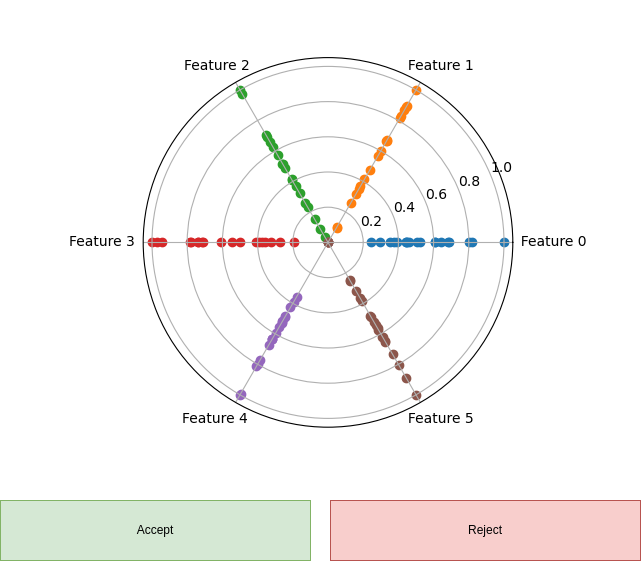
\includegraphics[width=0.8\textwidth]{figures/check_input_coverage.png}
\caption{"Check input coverage" mock-up form}
\end{figure}

\begin{table}[H]
\centering
\begin{tabularx}{\textwidth}{|X|c|c|c|c|}
\hline
\textbf{Step} & \textbf{O} & \textbf{CL} & \textbf{S} & \textbf{SC} \\
\hline
\textbf{1} \textbf{ACTOR} opens "Check input coverage" form. & & & & \\
\hline
\textbf{2} \textbf{SYSTEM} shows a radar scatter plot of the input distribution. & & & & \\
\hline
\textbf{3} \textbf{FOR EACH} radius in the radar scatter plot: & & & & \\
\hline
\textbf{3.1} \textbf{IF} the distribution is not uniform as expected. & & & & \\
\hline
\textbf{3.1.1} \textbf{THEN} the input coverage is not satisfied. & & & & \\
\hline
\textbf{4.1} \textbf{IF} the input coverage is satisfied. & & & & \\
\hline
\textbf{4.1.1} \textbf{ACTOR} clicks "Accept" button. & & & & \\
\hline
\textbf{4.2} \textbf{ELSE} & & & & \\
\hline
\textbf{4.2.1} \textbf{ACTOR} clicks "Reject" button. & & & & \\
\hline
\textbf{5} \textbf{SYSTEM} shows a confirmation dialog. & & & & \\
\hline
\textbf{6} \textbf{ACTOR} closes the form. & & & & \\
\hline
\multicolumn{4}{|r|}{Human task cost} & \\
\hline
\end{tabularx}
\caption{Detailed use case for "Check input coverage" task}
\label{table:check_input_coverage}
\end{table}

\subsection{Development system}

\subsubsection{Set iteration number}

\begin{figure}[H]
\centering
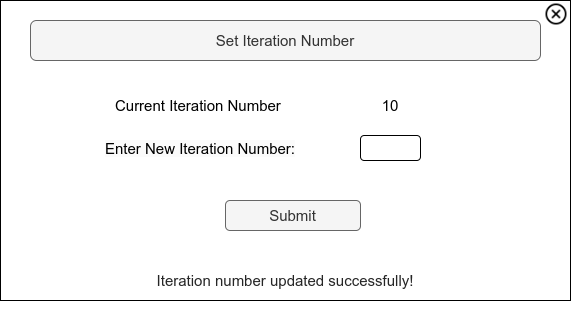
\includegraphics[width=0.8\textwidth]{figures/set_iteration_number.png}
\caption{"Set iteration number" mock-up form}
\end{figure}

\begin{table}[H]
\centering
\begin{tabularx}{\textwidth}{|X|c|c|c|c|}
\hline
\textbf{Step} & \textbf{O} & \textbf{CL} & \textbf{S} & \textbf{SC} \\
\hline
\textbf{1} \textbf{ACTOR} opens "Set Iteration Number" form. & & & & \\
\hline
\textbf{2} \textbf{SYSTEM} displays the current iteration number. & & & & \\
\hline
\textbf{3} \textbf{ACTOR} inputs the desired number of iterations. & & & & \\
\hline
\textbf{4} \textbf{ACTOR} clicks "Submit" button to confirm the iteration number. & & & & \\
\hline
\textbf{5} \textbf{SYSTEM} shows a confirmation dialog. & & & & \\
\hline
\textbf{6} \textbf{ACTOR} closes the form. & & & & \\
\hline
\multicolumn{4}{|r|}{Human task cost} & \\
\hline
\end{tabularx}
\caption{Detailed use case for "Set iteration number" task}
\label{table:set_iteration_number}
\end{table}

\subsubsection{Check learning plot}

\begin{table}[H]
\centering
\begin{tabularx}{\textwidth}{|X|c|c|c|c|}
\hline
\textbf{Step} & \textbf{O} & \textbf{CL} & \textbf{S} & \textbf{SC} \\
\hline
\textbf{1} \textbf{ACTOR} opens "Check training report" form. & & & & \\
\hline
\textbf{2} \textbf{SYSTEM} shows the training loss curve. & & & & \\
\hline
\textbf{3.1} \textbf{IF} the loss is flat for at least half of the iterations: & & & & \\
\hline
\textbf{3.1.1} \textbf{THEN} \textbf{ACTOR} clicks "Overfit" button. & & & & \\
\hline
\textbf{3.2} \textbf{IF} the loss is not flat at the end of the iterations: & & & & \\
\hline
\textbf{3.2.1} \textbf{THEN} \textbf{ACTOR} clicks "Underfit" button. & & & & \\
\hline
\textbf{3.3} \textbf{ELSE} & & & & \\
\hline
\textbf{3.3.1} \textbf{ACTOR} clicks "Approved" button. & & & & \\
\hline
\textbf{4} \textbf{SYSTEM} shows a confirmation dialog. & & & & \\
\hline
\textbf{5} \textbf{ACTOR} closes the form. & & & & \\
\hline
\multicolumn{4}{|r|}{Human task cost} & \\
\hline
\end{tabularx}
\caption{Detailed use case for "Check training report" task}
\label{table:check_training_report}
\end{table}

\subsubsection{Check validation report}

\begin{figure}[H]
\centering
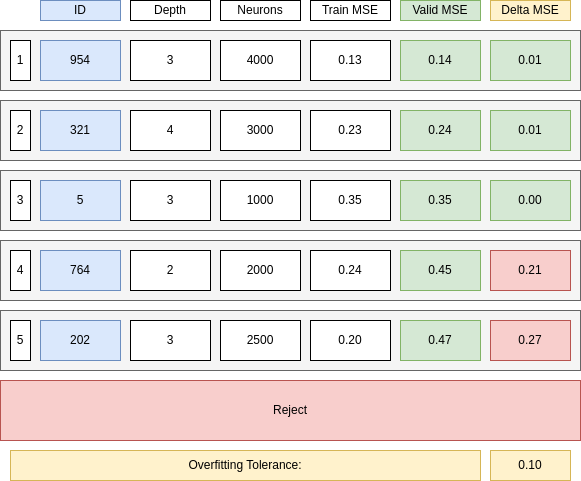
\includegraphics[width=0.8\textwidth]{figures/check_validation_report.png}
\caption{"Check validation report" mock-up form}
\end{figure}

\begin{table}[H]
\centering
\begin{tabularx}{\textwidth}{|X|c|c|c|c|}
\hline
\textbf{Step} & \textbf{O} & \textbf{CL} & \textbf{S} & \textbf{SC} \\
\hline
\textbf{1} \textbf{ACTOR} opens "Check validation report" form. & & & & \\
\hline
\textbf{2} \textbf{SYSTEM} shows the best 5 models sorted by increasing Validation Loss. & & & & \\
\hline
\textbf{3} \textbf{FOR EACH} model in the list: & & & & \\
\hline
\textbf{3.1} \textbf{IF} the model Validation Loss minus the Training Loss is less than the Overfitting Tolerance. & & & & \\
\hline
\textbf{3.1.1} \textbf{THEN} select the model as the Best Model. & & & & \\
\hline
\textbf{4} \textbf{FOR EACH} model in the list: & & & & \\
\hline
\textbf{4.1} \textbf{IF} the model is not the Best Model and the Validation Loss minus the Training Loss is less than the Overfitting Tolerance. & & & & \\
\hline
\textbf{4.1.1} \textbf{THEN} select the model as the Second Best Model. & & & & \\
\hline
\textbf{5.1} \textbf{IF} the Best Model is not selected. & & & & \\
\hline
\textbf{5.1.1} \textbf{ACTOR} clicks "Reject" button. & & & & \\
\hline
\textbf{5.2} \textbf{ELSE IF} the Second Best Model is not selected or the Validation Loss of the Second Best Model is one order of magnitude greater than the Validation Loss of the Best Model. & & & & \\
\hline
\textbf{5.2.1} \textbf{ACTOR} clicks on the Best Model. & & & & \\
\hline
\textbf{5.3} \textbf{ELSE} & & & & \\
\hline
\textbf{5.3.1} \textbf{ACTOR} clicks on the least complex model among the Best Model and the Second Best Model. & & & & \\
\hline
\textbf{6} \textbf{SYSTEM} shows a confirmation dialog. & & & & \\
\hline
\textbf{7} \textbf{ACTOR} closes the form. & & & & \\
\hline
\multicolumn{4}{|r|}{Human task cost} & \\
\hline
\end{tabularx}
\caption{Detailed use case for "Check validation report" task}
\label{table:check_validation_report}
\end{table}

\subsubsection{Check test results}

\begin{figure}[H]
\centering
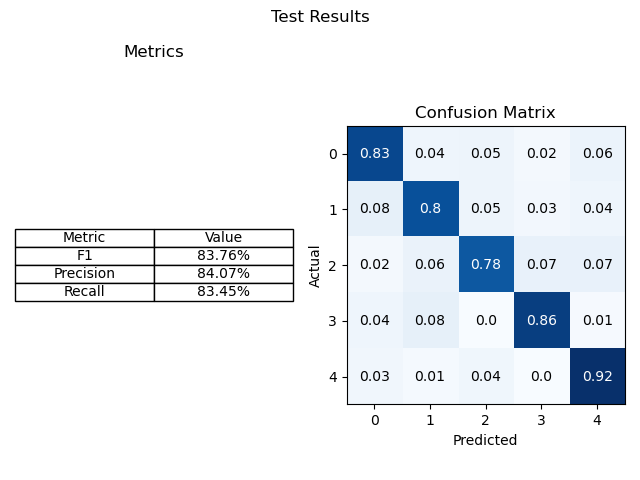
\includegraphics[width=0.8\textwidth]{figures/check_test_results.png}
\caption{"Check test results" mock-up form}
\end{figure}

\begin{table}[H]
\centering
\begin{tabularx}{\textwidth}{|X|c|c|c|c|}
\hline
\textbf{Step} & \textbf{O} & \textbf{CL} & \textbf{S} & \textbf{SC} \\
\hline
\textbf{1} \textbf{ACTOR} opens "Check test results" form. & & & & \\
\hline
\textbf{2} \textbf{SYSTEM} shows the test results. & & & & \\
\hline
\textbf{3} \textbf{ACTOR} checks if the difference between the test results and the validation results is within overfitting tolerance. & & & & \\
\hline
\textbf{4.1} \textbf{IF} the test results is not satisfactory. & & & & \\
\hline
\textbf{4.1.1} \textbf{ACTOR} clicks "Reject" button. & & & & \\
\hline
\textbf{4.2} \textbf{ELSE} & & & & \\
\hline
\textbf{4.2.1} \textbf{ACTOR} clicks "Approve" button. & & & & \\
\hline
\textbf{5} \textbf{SYSTEM} shows a confirmation dialog. & & & & \\
\hline
\textbf{6} \textbf{ACTOR} closes the form. & & & & \\
\hline
\multicolumn{4}{|r|}{Human task cost} & \\
\hline
\end{tabularx}
\caption{Detailed use case for "Check test results" task}
\label{table:check_test_results}
\end{table}


\subsection{Evaluation system}

\subsubsection{Evaluate classifier performance}

\begin{figure}[H]
\centering
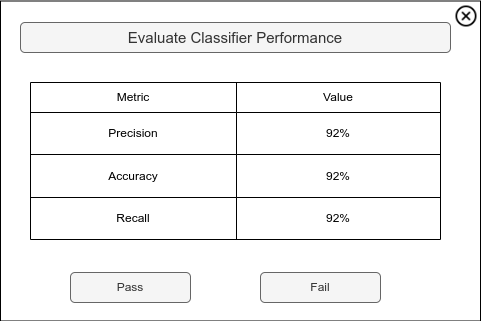
\includegraphics[width=0.8\textwidth]{figures/evaluate_classifier_performance.png}
\caption{"Evaluate Classifier Performance" mock-up form}
\end{figure}

\begin{table}[H]
\centering
\begin{tabularx}{\textwidth}{|X|c|c|c|c|}
\hline
\textbf{Step} & \textbf{O} & \textbf{CL} & \textbf{S} & \textbf{SC} \\
\hline
\textbf{1} \textbf{ACTOR} opens the "Evaluate Classifier Performance" form. & & & & \\
\hline
\textbf{2} \textbf{SYSTEM} displays a table of sessions with Expert Label (ground truth) and Classifier Label (predicted label). 
The difference between the labels (if any) represents an error. & & & & \\
\hline
\textbf{3} \textbf{ACTOR} reviews the table. & & & & \\
\hline
\textbf{3.1} \textbf{IF} the total errors or consecutive errors exceed their respective thresholds: & & & & \\
\hline
\textbf{3.1.1} \textbf{ACTOR} clicks the "Fail" button. & & & & \\
\hline
\textbf{3.2} \textbf{ELSE} & & & & \\
\hline
\textbf{3.2.1} \textbf{ACTOR} clicks the "Pass" button. & & & & \\
\hline
\textbf{4} \textbf{SYSTEM} shows a confirmation dialog. & & & & \\
\hline
\textbf{5} \textbf{ACTOR} closes the form. & & & & \\
\hline
\multicolumn{4}{|r|}{Human task cost} & \\
\hline
\end{tabularx}
\caption{Detailed use case for "Evaluate Classifier Performance" task}
\label{table:evaluate_classifier_performance}
\end{table}
